\section {The PCB}
\begin{figure}[h]
  \centering
  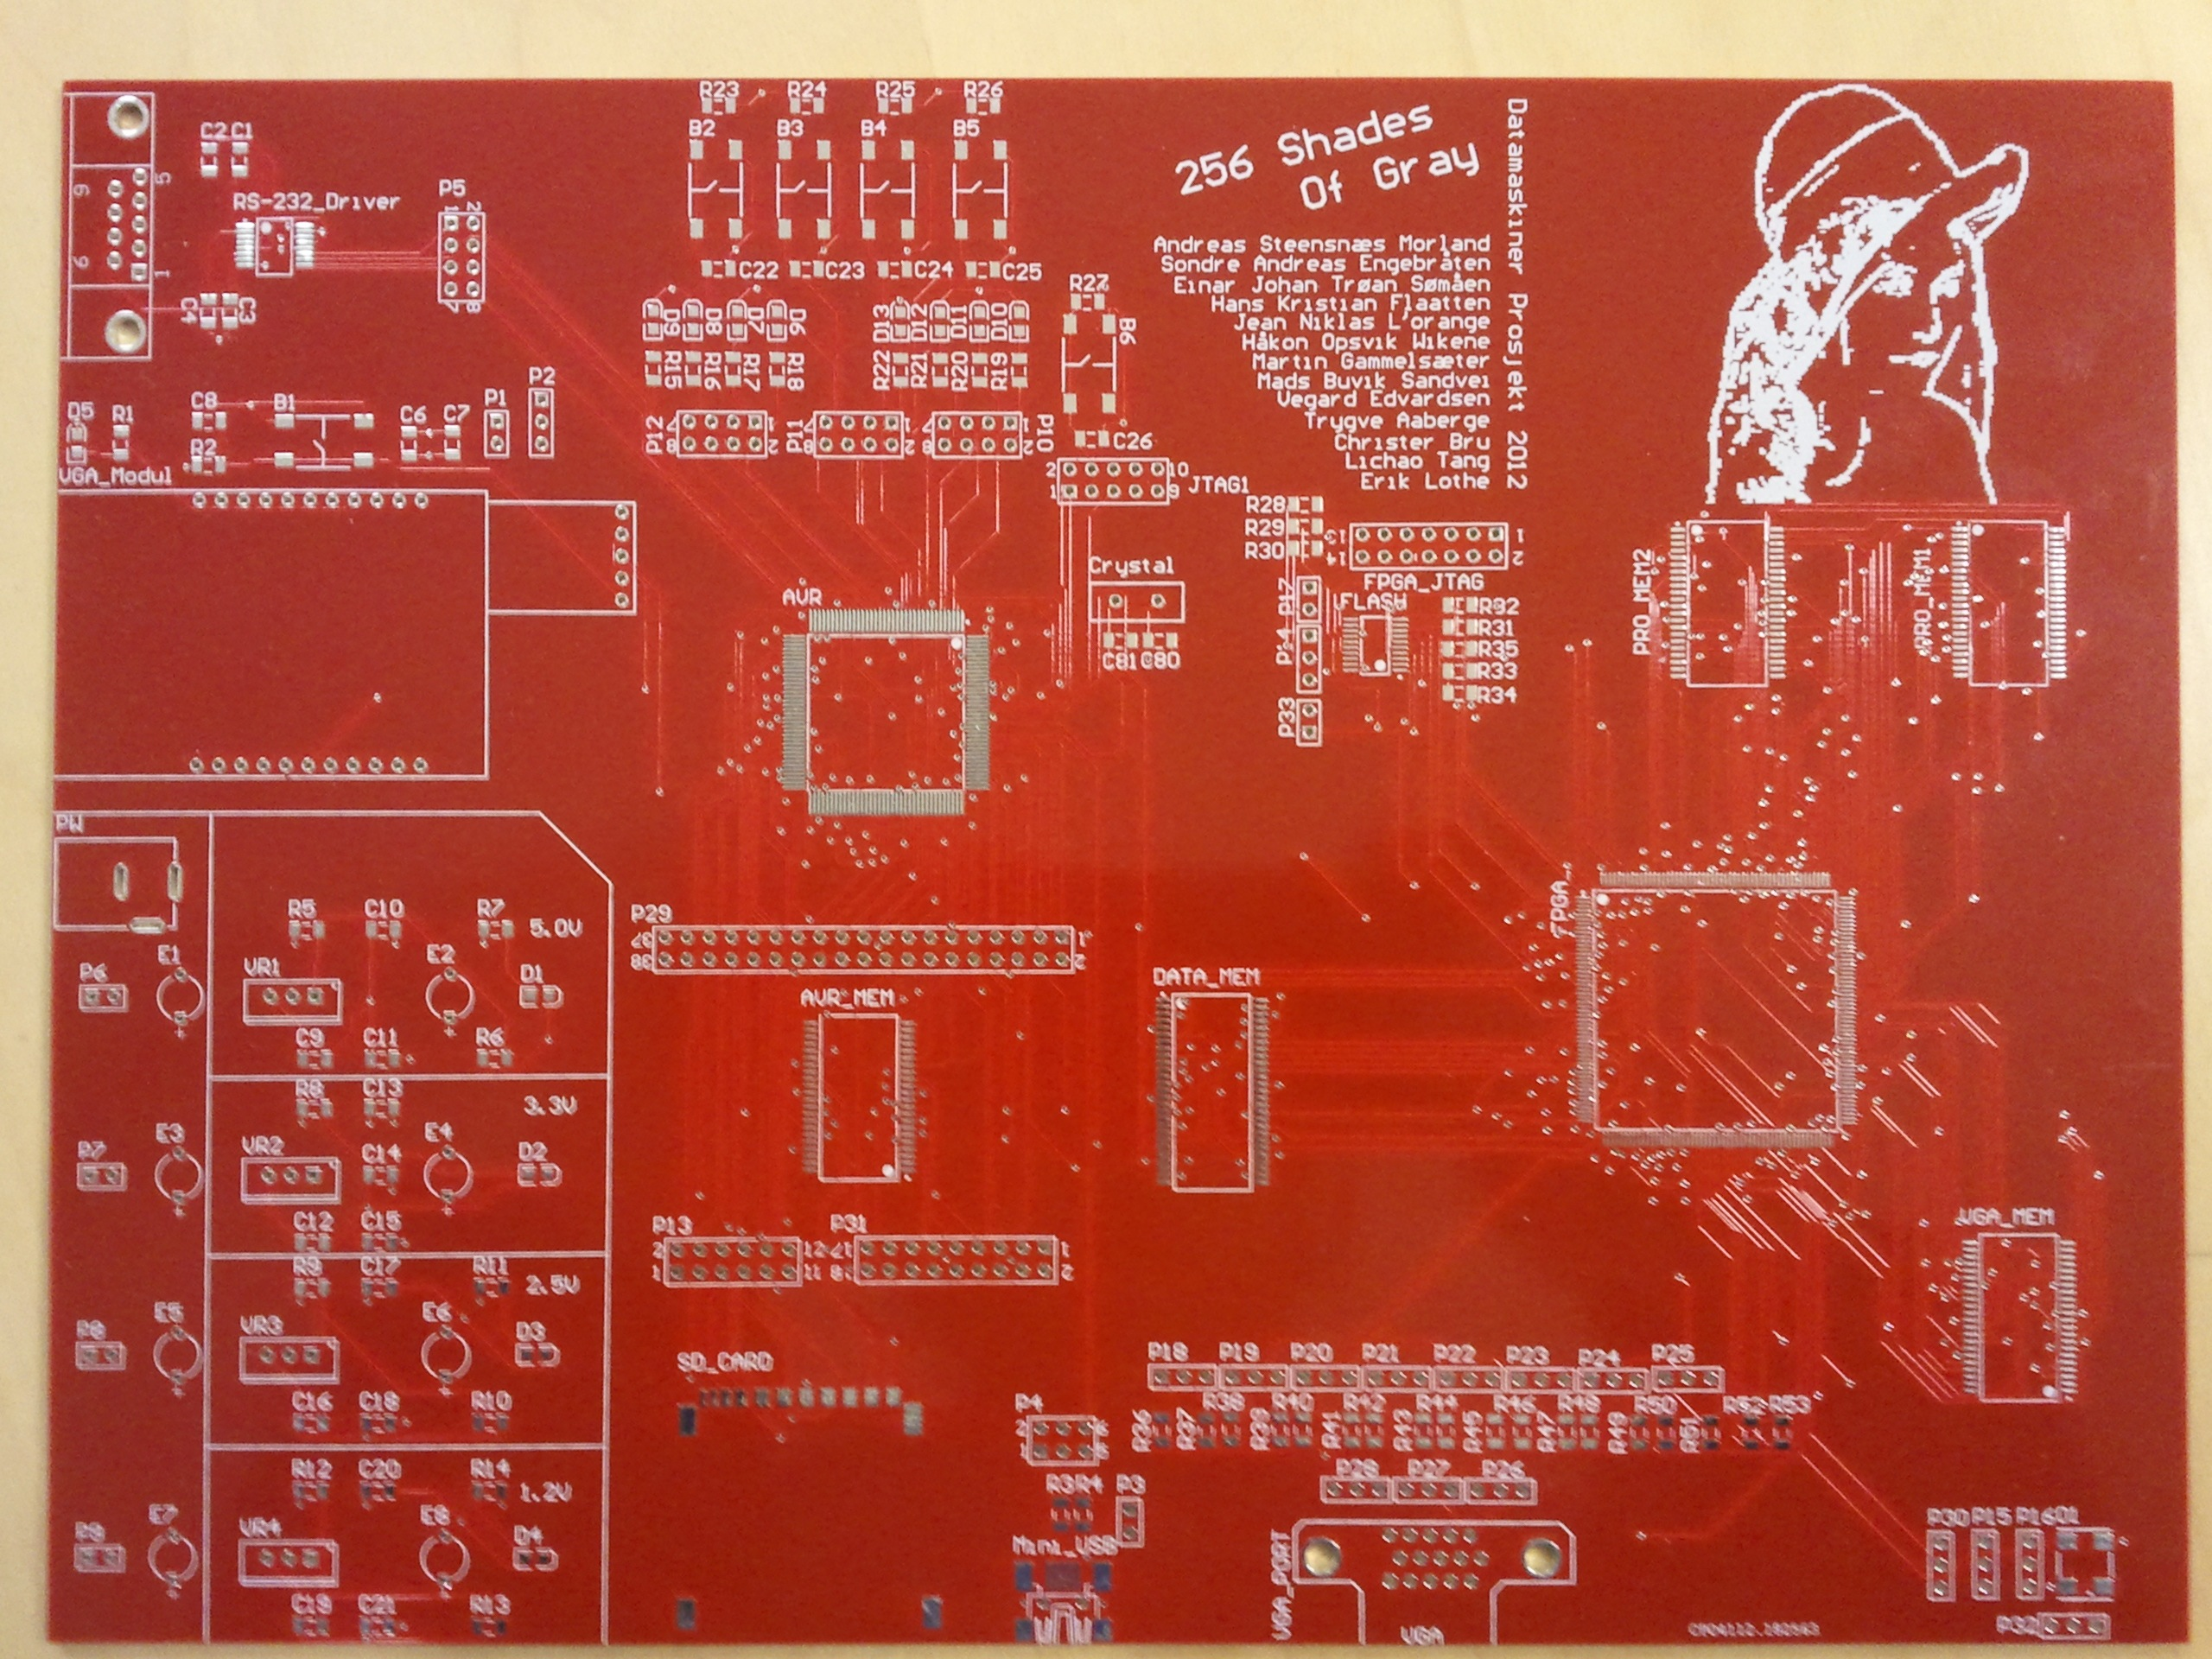
\includegraphics[width=\textwidth]{fig/pcb/pcbwithoutcomp}
  \caption{The PCB without Components}
  \label{fig:figurlabel}
\end{figure}
When the PCB finally arrived from production we started soldering, this proved to be a bit
more difficult than originally anticipated. First, we tested whether there were short circuit in our PCB. We used multimeter to test there was no current that goes from different layer. Then, we started to solder with the power supply part, and tested. \\
\begin{table}[h]
  \centering
  \begin{tabularx}{\textwidth}{l l l l}\toprule
    \thx{Test} & \thx{Result} & \thx{Passed} 
    \\ 
	 \midrule
    Power supply 12.0V               &Measured 12.045  & OK  \\	
\midrule
    Power supply 5.0V               &Measured 4.995  & OK  \\
    \midrule
    Power supply 3.3V                   & Measured 3.286 & OK  \\
    \midrule
    Power supply 2.5V                 & Measured 2.510 & OK \\
    \midrule
    Power supply 1.2V            & Measured 1.240 & OK  \\
    
    \bottomrule
  \end{tabularx}
  \caption{Results of power supply}
  \label{fig:pcb}
\end{table}
\\
Then we started with AVR, getting the AVR in place was particularly difficult,but after asked Gunnar we lent a glue stick to put some glue on it to get more friction, and thus avoided it moving away the instant we came close with the solder iron.

After about a days work we managed to destroy a pin on the AVR, and thus had to redo completely on a new board. The soldering of second board seemed to be greater than the first one, this time we started with the AVR and FPGA, because we didn't have enough spare components. After we finished the AVR, FPGA, and power supply parts, in order to check the PCB was working, the AVR and FPGA groups tested the PCB board without the capacitors, after both groups tested that they could connect to the AVR and FPGA respectively, we began to solder the rest part of the PCB.  

